\documentclass[1p]{elsarticle_modified}
%\bibliographystyle{elsarticle-num}

%\usepackage[colorlinks]{hyperref}
%\usepackage{abbrmath_seonhwa} %\Abb, \Ascr, \Acal ,\Abf, \Afrak
\usepackage{amsfonts}
\usepackage{amssymb}
\usepackage{amsmath}
\usepackage{amsthm}
\usepackage{scalefnt}
\usepackage{amsbsy}
\usepackage{kotex}
\usepackage{caption}
\usepackage{subfig}
\usepackage{color}
\usepackage{graphicx}
\usepackage{xcolor} %% white, black, red, green, blue, cyan, magenta, yellow
\usepackage{float}
\usepackage{setspace}
\usepackage{hyperref}

\usepackage{tikz}
\usetikzlibrary{arrows}

\usepackage{multirow}
\usepackage{array} % fixed length table
\usepackage{hhline}

%%%%%%%%%%%%%%%%%%%%%
\makeatletter
\renewcommand*\env@matrix[1][\arraystretch]{%
	\edef\arraystretch{#1}%
	\hskip -\arraycolsep
	\let\@ifnextchar\new@ifnextchar
	\array{*\c@MaxMatrixCols c}}
\makeatother %https://tex.stackexchange.com/questions/14071/how-can-i-increase-the-line-spacing-in-a-matrix
%%%%%%%%%%%%%%%

\usepackage[normalem]{ulem}

\newcommand{\msout}[1]{\ifmmode\text{\sout{\ensuremath{#1}}}\else\sout{#1}\fi}
%SOURCE: \msout is \stkout macro in https://tex.stackexchange.com/questions/20609/strikeout-in-math-mode

\newcommand{\cancel}[1]{
	\ifmmode
	{\color{red}\msout{#1}}
	\else
	{\color{red}\sout{#1}}
	\fi
}

\newcommand{\add}[1]{
	{\color{blue}\uwave{#1}}
}

\newcommand{\replace}[2]{
	\ifmmode
	{\color{red}\msout{#1}}{\color{blue}\uwave{#2}}
	\else
	{\color{red}\sout{#1}}{\color{blue}\uwave{#2}}
	\fi
}

\newcommand{\Sol}{\mathcal{S}} %segment
\newcommand{\D}{D} %diagram
\newcommand{\A}{\mathcal{A}} %arc


%%%%%%%%%%%%%%%%%%%%%%%%%%%%%5 test

\def\sl{\operatorname{\textup{SL}}(2,\Cbb)}
\def\psl{\operatorname{\textup{PSL}}(2,\Cbb)}
\def\quan{\mkern 1mu \triangleright \mkern 1mu}

\theoremstyle{definition}
\newtheorem{thm}{Theorem}[section]
\newtheorem{prop}[thm]{Proposition}
\newtheorem{lem}[thm]{Lemma}
\newtheorem{ques}[thm]{Question}
\newtheorem{cor}[thm]{Corollary}
\newtheorem{defn}[thm]{Definition}
\newtheorem{exam}[thm]{Example}
\newtheorem{rmk}[thm]{Remark}
\newtheorem{alg}[thm]{Algorithm}

\newcommand{\I}{\sqrt{-1}}
\begin{document}

%\begin{frontmatter}
%
%\title{Boundary parabolic representations of knots up to 8 crossings}
%
%%% Group authors per affiliation:
%\author{Yunhi Cho} 
%\address{Department of Mathematics, University of Seoul, Seoul, Korea}
%\ead{yhcho@uos.ac.kr}
%
%
%\author{Seonhwa Kim} %\fnref{s_kim}}
%\address{Center for Geometry and Physics, Institute for Basic Science, Pohang, 37673, Korea}
%\ead{ryeona17@ibs.re.kr}
%
%\author{Hyuk Kim}
%\address{Department of Mathematical Sciences, Seoul National University, Seoul 08826, Korea}
%\ead{hyukkim@snu.ac.kr}
%
%\author{Seokbeom Yoon}
%\address{Department of Mathematical Sciences, Seoul National University, Seoul, 08826,  Korea}
%\ead{sbyoon15@snu.ac.kr}
%
%\begin{abstract}
%We find all boundary parabolic representation of knots up to 8 crossings.
%
%\end{abstract}
%\begin{keyword}
%    \MSC[2010] 57M25 
%\end{keyword}
%
%\end{frontmatter}

%\linenumbers
%\tableofcontents
%
\newcommand\colored[1]{\textcolor{white}{\rule[-0.35ex]{0.8em}{1.4ex}}\kern-0.8em\color{red} #1}%
%\newcommand\colored[1]{\textcolor{white}{ #1}\kern-2.17ex	\textcolor{white}{ #1}\kern-1.81ex	\textcolor{white}{ #1}\kern-2.15ex\color{red}#1	}

{\Large $\underline{12n_{0704}~(K12n_{0704})}$}

\setlength{\tabcolsep}{10pt}
\renewcommand{\arraystretch}{1.6}
\vspace{1cm}\begin{tabular}{m{100pt}>{\centering\arraybackslash}m{274pt}}
\multirow{5}{120pt}{
	\centering
	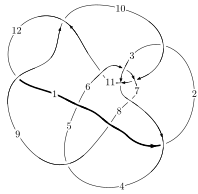
\includegraphics[width=112pt]{../../../GIT/diagram.site/Diagrams/png/2793_12n_0704.png}\\
\ \ \ A knot diagram\footnotemark}&
\allowdisplaybreaks
\textbf{Linearized knot diagam} \\
\cline{2-2}
 &
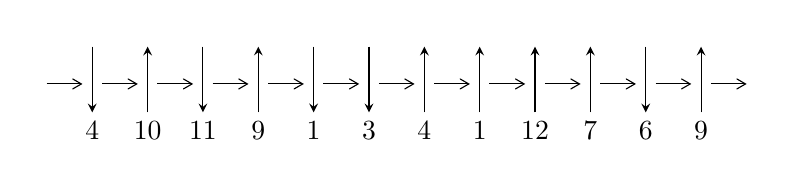
\begin{tikzpicture}[x=20pt, y=17pt]
	% nodes
	\node (C0) at (0, 0) {};
	\node (C1) at (1, 0) {};
	\node (C1U) at (1, +1) {};
	\node (C1D) at (1, -1) {4};

	\node (C2) at (2, 0) {};
	\node (C2U) at (2, +1) {};
	\node (C2D) at (2, -1) {10};

	\node (C3) at (3, 0) {};
	\node (C3U) at (3, +1) {};
	\node (C3D) at (3, -1) {11};

	\node (C4) at (4, 0) {};
	\node (C4U) at (4, +1) {};
	\node (C4D) at (4, -1) {9};

	\node (C5) at (5, 0) {};
	\node (C5U) at (5, +1) {};
	\node (C5D) at (5, -1) {1};

	\node (C6) at (6, 0) {};
	\node (C6U) at (6, +1) {};
	\node (C6D) at (6, -1) {3};

	\node (C7) at (7, 0) {};
	\node (C7U) at (7, +1) {};
	\node (C7D) at (7, -1) {4};

	\node (C8) at (8, 0) {};
	\node (C8U) at (8, +1) {};
	\node (C8D) at (8, -1) {1};

	\node (C9) at (9, 0) {};
	\node (C9U) at (9, +1) {};
	\node (C9D) at (9, -1) {12};

	\node (C10) at (10, 0) {};
	\node (C10U) at (10, +1) {};
	\node (C10D) at (10, -1) {7};

	\node (C11) at (11, 0) {};
	\node (C11U) at (11, +1) {};
	\node (C11D) at (11, -1) {6};

	\node (C12) at (12, 0) {};
	\node (C12U) at (12, +1) {};
	\node (C12D) at (12, -1) {9};
	\node (C13) at (13, 0) {};

	% arrows
	\draw[->,>={angle 60}]
	(C0) edge (C1) (C1) edge (C2) (C2) edge (C3) (C3) edge (C4) (C4) edge (C5) (C5) edge (C6) (C6) edge (C7) (C7) edge (C8) (C8) edge (C9) (C9) edge (C10) (C10) edge (C11) (C11) edge (C12) (C12) edge (C13) ;	\draw[->,>=stealth]
	(C1U) edge (C1D) (C2D) edge (C2U) (C3U) edge (C3D) (C4D) edge (C4U) (C5U) edge (C5D) (C6U) edge (C6D) (C7D) edge (C7U) (C8D) edge (C8U) (C9D) edge (C9U) (C10D) edge (C10U) (C11U) edge (C11D) (C12D) edge (C12U) ;
	\end{tikzpicture} \\
\hhline{~~} \\& 
\textbf{Solving Sequence} \\ \cline{2-2} 
 &
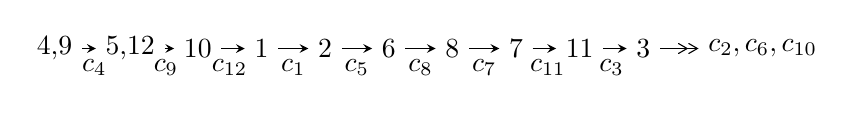
\begin{tikzpicture}[x=23pt, y=7pt]
	% node
	\node (A0) at (-1/8, 0) {4,9};
	\node (A1) at (17/16, 0) {5,12};
	\node (A2) at (17/8, 0) {10};
	\node (A3) at (25/8, 0) {1};
	\node (A4) at (33/8, 0) {2};
	\node (A5) at (41/8, 0) {6};
	\node (A6) at (49/8, 0) {8};
	\node (A7) at (57/8, 0) {7};
	\node (A8) at (65/8, 0) {11};
	\node (A9) at (73/8, 0) {3};
	\node (C1) at (1/2, -1) {$c_{4}$};
	\node (C2) at (13/8, -1) {$c_{9}$};
	\node (C3) at (21/8, -1) {$c_{12}$};
	\node (C4) at (29/8, -1) {$c_{1}$};
	\node (C5) at (37/8, -1) {$c_{5}$};
	\node (C6) at (45/8, -1) {$c_{8}$};
	\node (C7) at (53/8, -1) {$c_{7}$};
	\node (C8) at (61/8, -1) {$c_{11}$};
	\node (C9) at (69/8, -1) {$c_{3}$};
	\node (A10) at (11, 0) {$c_{2},c_{6},c_{10}$};

	% edge
	\draw[->,>=stealth]	
	(A0) edge (A1) (A1) edge (A2) (A2) edge (A3) (A3) edge (A4) (A4) edge (A5) (A5) edge (A6) (A6) edge (A7) (A7) edge (A8) (A8) edge (A9) ;
	\draw[->>,>={angle 60}]	
	(A9) edge (A10);
\end{tikzpicture} \\ 

\end{tabular} \\

\footnotetext{
The image of knot diagram is generated by the software ``\textbf{Draw programme}" developed by Andrew Bartholomew(\url{http://www.layer8.co.uk/maths/draw/index.htm\#Running-draw}), where we modified some parts for our purpose(\url{https://github.com/CATsTAILs/LinksPainter}).
}\phantom \\ \newline 
\centering \textbf{Ideals for irreducible components\footnotemark of $X_{\text{par}}$} 
 
\begin{align*}
I^u_{1}&=\langle 
1.19445\times10^{198} u^{45}-6.74601\times10^{197} u^{44}+\cdots+4.55141\times10^{201} b-1.33536\times10^{201},\\
\phantom{I^u_{1}}&\phantom{= \langle  }1.06146\times10^{200} u^{45}+1.69938\times10^{199} u^{44}+\cdots+1.77505\times10^{203} a-2.99606\times10^{203},\\
\phantom{I^u_{1}}&\phantom{= \langle  }u^{46}+56 u^{44}+\cdots-1378 u+507\rangle \\
I^u_{2}&=\langle 
788638025662 u^{15}-78518326905455 u^{14}+\cdots+919477490510109 b-419677061820201,\\
\phantom{I^u_{2}}&\phantom{= \langle  }73623372272275 u^{15}-47637302039197 u^{14}+\cdots+919477490510109 a+2632097779359569,\\
\phantom{I^u_{2}}&\phantom{= \langle  }u^{16}+u^{15}+\cdots+15 u+9\rangle \\
\\
\end{align*}
\raggedright * 2 irreducible components of $\dim_{\mathbb{C}}=0$, with total 62 representations.\\
\footnotetext{All coefficients of polynomials are rational numbers. But the coefficients are sometimes approximated in decimal forms when there is not enough margin.}
\newpage
\renewcommand{\arraystretch}{1}
\centering \section*{I. $I^u_{1}= \langle 1.19\times10^{198} u^{45}-6.75\times10^{197} u^{44}+\cdots+4.55\times10^{201} b-1.34\times10^{201},\;1.06\times10^{200} u^{45}+1.70\times10^{199} u^{44}+\cdots+1.78\times10^{203} a-3.00\times10^{203},\;u^{46}+56 u^{44}+\cdots-1378 u+507 \rangle$}
\flushleft \textbf{(i) Arc colorings}\\
\begin{tabular}{m{7pt} m{180pt} m{7pt} m{180pt} }
\flushright $a_{4}=$&$\begin{pmatrix}1\\0\end{pmatrix}$ \\
\flushright $a_{9}=$&$\begin{pmatrix}0\\u\end{pmatrix}$ \\
\flushright $a_{5}=$&$\begin{pmatrix}1\\- u^2\end{pmatrix}$ \\
\flushright $a_{12}=$&$\begin{pmatrix}-0.000597989 u^{45}-0.0000957369 u^{44}+\cdots-1.97693 u+1.68787\\-0.000262435 u^{45}+0.000148218 u^{44}+\cdots+0.754607 u+0.293395\end{pmatrix}$ \\
\flushright $a_{10}=$&$\begin{pmatrix}-0.000625366 u^{45}-0.000355332 u^{44}+\cdots-0.368332 u+1.08941\\0.0000695995 u^{45}+0.000148080 u^{44}+\cdots+1.20417 u+0.198918\end{pmatrix}$ \\
\flushright $a_{1}=$&$\begin{pmatrix}-0.000597989 u^{45}-0.0000957369 u^{44}+\cdots-1.97693 u+1.68787\\-0.000174434 u^{45}+0.000154808 u^{44}+\cdots+0.583352 u+0.244856\end{pmatrix}$ \\
\flushright $a_{2}=$&$\begin{pmatrix}-0.000423555 u^{45}-0.000250544 u^{44}+\cdots-2.56028 u+1.44302\\-0.000174434 u^{45}+0.000154808 u^{44}+\cdots+0.583352 u+0.244856\end{pmatrix}$ \\
\flushright $a_{6}=$&$\begin{pmatrix}-0.000392342 u^{45}+0.0000695995 u^{44}+\cdots+0.902157 u+1.74482\\0.000138440 u^{45}+0.0000385594 u^{44}+\cdots+0.267201 u+0.0758209\end{pmatrix}$ \\
\flushright $a_{8}=$&$\begin{pmatrix}0.000625366 u^{45}+0.000355332 u^{44}+\cdots+0.368332 u-1.08941\\-0.0000243237 u^{45}-0.000122334 u^{44}+\cdots+0.623241 u-0.0187641\end{pmatrix}$ \\
\flushright $a_{7}=$&$\begin{pmatrix}0.000649690 u^{45}+0.000477667 u^{44}+\cdots-0.254909 u-1.07065\\-0.0000243237 u^{45}-0.000122334 u^{44}+\cdots+0.623241 u-0.0187641\end{pmatrix}$ \\
\flushright $a_{11}=$&$\begin{pmatrix}-0.000621843 u^{45}-0.0000319284 u^{44}+\cdots+1.04140 u+2.54422\\-0.000195680 u^{45}+0.0000193035 u^{44}+\cdots+1.10047 u+0.158773\end{pmatrix}$ \\
\flushright $a_{3}=$&$\begin{pmatrix}0.000304275 u^{45}-0.000150311 u^{44}+\cdots-2.53168 u+0.571523\\-0.000414380 u^{45}-0.0000218287 u^{44}+\cdots-0.337787 u+0.0757931\end{pmatrix}$\\&\end{tabular}
\flushleft \textbf{(ii) Obstruction class $= -1$}\\~\\
\flushleft \textbf{(iii) Cusp Shapes $= -0.00268732 u^{45}+0.000514392 u^{44}+\cdots-6.90355 u+4.66863$}\\~\\
\newpage\renewcommand{\arraystretch}{1}
\flushleft \textbf{(iv) u-Polynomials at the component}\newline \\
\begin{tabular}{m{50pt}|m{274pt}}
Crossings & \hspace{64pt}u-Polynomials at each crossing \\
\hline $$\begin{aligned}c_{1}\end{aligned}$$&$\begin{aligned}
&u^{46}+9 u^{45}+\cdots-598194 u+53041
\end{aligned}$\\
\hline $$\begin{aligned}c_{2}\end{aligned}$$&$\begin{aligned}
&u^{46}+14 u^{44}+\cdots-11 u+1
\end{aligned}$\\
\hline $$\begin{aligned}c_{3}\end{aligned}$$&$\begin{aligned}
&u^{46}-3 u^{45}+\cdots-23 u+3
\end{aligned}$\\
\hline $$\begin{aligned}c_{4}\end{aligned}$$&$\begin{aligned}
&u^{46}+56 u^{44}+\cdots-1378 u+507
\end{aligned}$\\
\hline $$\begin{aligned}c_{5}\end{aligned}$$&$\begin{aligned}
&u^{46}-2 u^{45}+\cdots-250 u+1279
\end{aligned}$\\
\hline $$\begin{aligned}c_{6}\end{aligned}$$&$\begin{aligned}
&u^{46}+5 u^{45}+\cdots-9 u+1
\end{aligned}$\\
\hline $$\begin{aligned}c_{7}\end{aligned}$$&$\begin{aligned}
&u^{46}+15 u^{44}+\cdots-3108 u+149
\end{aligned}$\\
\hline $$\begin{aligned}c_{8},c_{9},c_{12}\end{aligned}$$&$\begin{aligned}
&u^{46}+33 u^{44}+\cdots-141 u+19
\end{aligned}$\\
\hline $$\begin{aligned}c_{10}\end{aligned}$$&$\begin{aligned}
&u^{46}-5 u^{45}+\cdots-51 u+31
\end{aligned}$\\
\hline $$\begin{aligned}c_{11}\end{aligned}$$&$\begin{aligned}
&u^{46}- u^{45}+\cdots+65 u+49
\end{aligned}$\\
\hline
\end{tabular}\\~\\
\newpage\renewcommand{\arraystretch}{1}
\flushleft \textbf{(v) Riley Polynomials at the component}\newline \\
\begin{tabular}{m{50pt}|m{274pt}}
Crossings & \hspace{64pt}Riley Polynomials at each crossing \\
\hline $$\begin{aligned}c_{1}\end{aligned}$$&$\begin{aligned}
&y^{46}-93 y^{45}+\cdots-17713407268 y+2813347681
\end{aligned}$\\
\hline $$\begin{aligned}c_{2}\end{aligned}$$&$\begin{aligned}
&y^{46}+28 y^{45}+\cdots+261 y+1
\end{aligned}$\\
\hline $$\begin{aligned}c_{3}\end{aligned}$$&$\begin{aligned}
&y^{46}+3 y^{45}+\cdots+5 y+9
\end{aligned}$\\
\hline $$\begin{aligned}c_{4}\end{aligned}$$&$\begin{aligned}
&y^{46}+112 y^{45}+\cdots+2295020 y+257049
\end{aligned}$\\
\hline $$\begin{aligned}c_{5}\end{aligned}$$&$\begin{aligned}
&y^{46}-108 y^{45}+\cdots-67250928 y+1635841
\end{aligned}$\\
\hline $$\begin{aligned}c_{6}\end{aligned}$$&$\begin{aligned}
&y^{46}+3 y^{45}+\cdots+9 y+1
\end{aligned}$\\
\hline $$\begin{aligned}c_{7}\end{aligned}$$&$\begin{aligned}
&y^{46}+30 y^{45}+\cdots-4374634 y+22201
\end{aligned}$\\
\hline $$\begin{aligned}c_{8},c_{9},c_{12}\end{aligned}$$&$\begin{aligned}
&y^{46}+66 y^{45}+\cdots+8809 y+361
\end{aligned}$\\
\hline $$\begin{aligned}c_{10}\end{aligned}$$&$\begin{aligned}
&y^{46}+13 y^{45}+\cdots+21765 y+961
\end{aligned}$\\
\hline $$\begin{aligned}c_{11}\end{aligned}$$&$\begin{aligned}
&y^{46}+19 y^{45}+\cdots+55653 y+2401
\end{aligned}$\\
\hline
\end{tabular}\\~\\
\newpage\flushleft \textbf{(vi) Complex Volumes and Cusp Shapes}
$$\begin{array}{c|c|c}  
\text{Solutions to }I^u_{1}& \I (\text{vol} + \sqrt{-1}CS) & \text{Cusp shape}\\
 \hline 
\begin{aligned}
u &= -0.722623 + 0.663783 I \\
a &= -0.189781 + 1.081440 I \\
b &= -0.761905 + 0.077110 I\end{aligned}
 & -4.43282 + 1.52715 I & -7.37334 - 5.22015 I \\ \hline\begin{aligned}
u &= -0.722623 - 0.663783 I \\
a &= -0.189781 - 1.081440 I \\
b &= -0.761905 - 0.077110 I\end{aligned}
 & -4.43282 - 1.52715 I & -7.37334 + 5.22015 I \\ \hline\begin{aligned}
u &= \phantom{-}1.042020 + 0.291189 I \\
a &= \phantom{-}0.311194 + 0.202668 I \\
b &= \phantom{-}0.527721 + 0.608546 I\end{aligned}
 & \phantom{-}1.89860 + 0.93839 I & -4.03451 + 1.19726 I \\ \hline\begin{aligned}
u &= \phantom{-}1.042020 - 0.291189 I \\
a &= \phantom{-}0.311194 - 0.202668 I \\
b &= \phantom{-}0.527721 - 0.608546 I\end{aligned}
 & \phantom{-}1.89860 - 0.93839 I & -4.03451 - 1.19726 I \\ \hline\begin{aligned}
u &= -0.594177 + 0.677482 I \\
a &= \phantom{-}0.97182 - 1.32120 I \\
b &= -0.344145 - 0.034677 I\end{aligned}
 & -4.23209 + 3.88598 I & -4.75603 - 4.49965 I \\ \hline\begin{aligned}
u &= -0.594177 - 0.677482 I \\
a &= \phantom{-}0.97182 + 1.32120 I \\
b &= -0.344145 + 0.034677 I\end{aligned}
 & -4.23209 - 3.88598 I & -4.75603 + 4.49965 I \\ \hline\begin{aligned}
u &= \phantom{-}0.181031 + 0.824245 I \\
a &= -0.373014 + 0.986862 I \\
b &= \phantom{-}0.386192 - 0.053287 I\end{aligned}
 & \phantom{-}0.75821 + 4.93973 I & \phantom{-}1.37497 - 6.10201 I \\ \hline\begin{aligned}
u &= \phantom{-}0.181031 - 0.824245 I \\
a &= -0.373014 - 0.986862 I \\
b &= \phantom{-}0.386192 + 0.053287 I\end{aligned}
 & \phantom{-}0.75821 - 4.93973 I & \phantom{-}1.37497 + 6.10201 I \\ \hline\begin{aligned}
u &= -0.168414 + 0.786367 I \\
a &= -1.019670 + 0.047056 I \\
b &= -0.890177 + 0.606122 I\end{aligned}
 & -4.06154 - 0.13020 I & -4.76095 - 0.53915 I \\ \hline\begin{aligned}
u &= -0.168414 - 0.786367 I \\
a &= -1.019670 - 0.047056 I \\
b &= -0.890177 - 0.606122 I\end{aligned}
 & -4.06154 + 0.13020 I & -4.76095 + 0.53915 I\\
 \hline 
 \end{array}$$\newpage$$\begin{array}{c|c|c}  
\text{Solutions to }I^u_{1}& \I (\text{vol} + \sqrt{-1}CS) & \text{Cusp shape}\\
 \hline 
\begin{aligned}
u &= \phantom{-}0.685524 + 0.242386 I \\
a &= \phantom{-}0.634928 + 0.396219 I \\
b &= \phantom{-}0.266521 + 0.975007 I\end{aligned}
 & \phantom{-}1.64805 + 1.08045 I & \phantom{-}3.15096 - 7.04605 I \\ \hline\begin{aligned}
u &= \phantom{-}0.685524 - 0.242386 I \\
a &= \phantom{-}0.634928 - 0.396219 I \\
b &= \phantom{-}0.266521 - 0.975007 I\end{aligned}
 & \phantom{-}1.64805 - 1.08045 I & \phantom{-}3.15096 + 7.04605 I \\ \hline\begin{aligned}
u &= -0.606976 + 0.353597 I \\
a &= \phantom{-}1.06341 - 1.70650 I \\
b &= \phantom{-}0.169419 - 1.237650 I\end{aligned}
 & -4.39199 + 5.06705 I & -1.75956 - 6.04792 I \\ \hline\begin{aligned}
u &= -0.606976 - 0.353597 I \\
a &= \phantom{-}1.06341 + 1.70650 I \\
b &= \phantom{-}0.169419 + 1.237650 I\end{aligned}
 & -4.39199 - 5.06705 I & -1.75956 + 6.04792 I \\ \hline\begin{aligned}
u &= \phantom{-}0.082102 + 0.677726 I \\
a &= \phantom{-}0.469990 - 0.277050 I \\
b &= -0.29228 - 1.51820 I\end{aligned}
 & \phantom{-}3.41907 - 4.27710 I & -1.86663 - 0.85536 I \\ \hline\begin{aligned}
u &= \phantom{-}0.082102 - 0.677726 I \\
a &= \phantom{-}0.469990 + 0.277050 I \\
b &= -0.29228 + 1.51820 I\end{aligned}
 & \phantom{-}3.41907 + 4.27710 I & -1.86663 + 0.85536 I \\ \hline\begin{aligned}
u &= -0.099218 + 0.655160 I \\
a &= \phantom{-}1.85892 + 0.20385 I \\
b &= -1.099660 + 0.530114 I\end{aligned}
 & -2.02807 + 0.89669 I & -0.59333 - 2.63444 I \\ \hline\begin{aligned}
u &= -0.099218 - 0.655160 I \\
a &= \phantom{-}1.85892 - 0.20385 I \\
b &= -1.099660 - 0.530114 I\end{aligned}
 & -2.02807 - 0.89669 I & -0.59333 + 2.63444 I \\ \hline\begin{aligned}
u &= \phantom{-}0.213548 + 0.536576 I \\
a &= \phantom{-}1.94510 - 0.08651 I \\
b &= \phantom{-}0.391610 + 0.666555 I\end{aligned}
 & -1.18834 + 2.94575 I & \phantom{-}2.79513 - 7.62929 I \\ \hline\begin{aligned}
u &= \phantom{-}0.213548 - 0.536576 I \\
a &= \phantom{-}1.94510 + 0.08651 I \\
b &= \phantom{-}0.391610 - 0.666555 I\end{aligned}
 & -1.18834 - 2.94575 I & \phantom{-}2.79513 + 7.62929 I\\
 \hline 
 \end{array}$$\newpage$$\begin{array}{c|c|c}  
\text{Solutions to }I^u_{1}& \I (\text{vol} + \sqrt{-1}CS) & \text{Cusp shape}\\
 \hline 
\begin{aligned}
u &= -0.225474 + 0.520584 I \\
a &= \phantom{-}0.860068 + 0.132577 I \\
b &= -0.575467 + 0.297341 I\end{aligned}
 & -1.20487 + 1.08188 I & -2.86879 - 1.93861 I \\ \hline\begin{aligned}
u &= -0.225474 - 0.520584 I \\
a &= \phantom{-}0.860068 - 0.132577 I \\
b &= -0.575467 - 0.297341 I\end{aligned}
 & -1.20487 - 1.08188 I & -2.86879 + 1.93861 I \\ \hline\begin{aligned}
u &= -0.529336 + 0.126590 I \\
a &= -0.73767 + 1.92374 I \\
b &= -0.833828 + 0.084948 I\end{aligned}
 & -3.13560 - 2.98726 I & -2.43600 + 6.69169 I \\ \hline\begin{aligned}
u &= -0.529336 - 0.126590 I \\
a &= -0.73767 - 1.92374 I \\
b &= -0.833828 - 0.084948 I\end{aligned}
 & -3.13560 + 2.98726 I & -2.43600 - 6.69169 I \\ \hline\begin{aligned}
u &= \phantom{-}0.362920 + 0.366463 I \\
a &= \phantom{-}0.70009 + 2.45399 I \\
b &= \phantom{-}0.875473 - 0.158897 I\end{aligned}
 & -3.13163 - 10.16720 I & -0.48934 + 7.57078 I \\ \hline\begin{aligned}
u &= \phantom{-}0.362920 - 0.366463 I \\
a &= \phantom{-}0.70009 - 2.45399 I \\
b &= \phantom{-}0.875473 + 0.158897 I\end{aligned}
 & -3.13163 + 10.16720 I & -0.48934 - 7.57078 I \\ \hline\begin{aligned}
u &= -1.47983 + 0.30015 I \\
a &= -0.113526 + 0.386179 I \\
b &= \phantom{-}0.466727 + 0.213716 I\end{aligned}
 & \phantom{-}2.38652 - 5.13357 I & \phantom{-0.000000 } 0 \\ \hline\begin{aligned}
u &= -1.47983 - 0.30015 I \\
a &= -0.113526 - 0.386179 I \\
b &= \phantom{-}0.466727 - 0.213716 I\end{aligned}
 & \phantom{-}2.38652 + 5.13357 I & \phantom{-0.000000 } 0 \\ \hline\begin{aligned}
u &= \phantom{-}0.206753 + 0.194399 I \\
a &= \phantom{-}2.05172 - 0.92917 I \\
b &= \phantom{-}0.347573 + 0.385865 I\end{aligned}
 & \phantom{-}1.35869 + 0.69751 I & \phantom{-}4.29607 - 0.54875 I \\ \hline\begin{aligned}
u &= \phantom{-}0.206753 - 0.194399 I \\
a &= \phantom{-}2.05172 + 0.92917 I \\
b &= \phantom{-}0.347573 - 0.385865 I\end{aligned}
 & \phantom{-}1.35869 - 0.69751 I & \phantom{-}4.29607 + 0.54875 I\\
 \hline 
 \end{array}$$\newpage$$\begin{array}{c|c|c}  
\text{Solutions to }I^u_{1}& \I (\text{vol} + \sqrt{-1}CS) & \text{Cusp shape}\\
 \hline 
\begin{aligned}
u &= \phantom{-}1.82791 + 0.18540 I \\
a &= \phantom{-}0.095317 - 0.729148 I \\
b &= -0.550395 - 1.005790 I\end{aligned}
 & -1.73016 + 2.21015 I & \phantom{-0.000000 } 0 \\ \hline\begin{aligned}
u &= \phantom{-}1.82791 - 0.18540 I \\
a &= \phantom{-}0.095317 + 0.729148 I \\
b &= -0.550395 + 1.005790 I\end{aligned}
 & -1.73016 - 2.21015 I & \phantom{-0.000000 } 0 \\ \hline\begin{aligned}
u &= -0.19250 + 2.63308 I \\
a &= \phantom{-}0.671878 - 0.103363 I \\
b &= -2.71999 + 0.09262 I\end{aligned}
 & -11.36540 + 5.64381 I & \phantom{-0.000000 } 0 \\ \hline\begin{aligned}
u &= -0.19250 - 2.63308 I \\
a &= \phantom{-}0.671878 + 0.103363 I \\
b &= -2.71999 - 0.09262 I\end{aligned}
 & -11.36540 - 5.64381 I & \phantom{-0.000000 } 0 \\ \hline\begin{aligned}
u &= \phantom{-}0.30985 + 2.75631 I \\
a &= \phantom{-}0.666351 + 0.066193 I \\
b &= -2.79148 + 0.01630 I\end{aligned}
 & -17.1201 + 5.1887 I & \phantom{-0.000000 } 0 \\ \hline\begin{aligned}
u &= \phantom{-}0.30985 - 2.75631 I \\
a &= \phantom{-}0.666351 - 0.066193 I \\
b &= -2.79148 - 0.01630 I\end{aligned}
 & -17.1201 - 5.1887 I & \phantom{-0.000000 } 0 \\ \hline\begin{aligned}
u &= -0.49972 + 2.82464 I \\
a &= -0.642407 + 0.112172 I \\
b &= \phantom{-}2.42127 + 0.01216 I\end{aligned}
 & -14.4376 + 0.6038 I & \phantom{-0.000000 } 0 \\ \hline\begin{aligned}
u &= -0.49972 - 2.82464 I \\
a &= -0.642407 - 0.112172 I \\
b &= \phantom{-}2.42127 - 0.01216 I\end{aligned}
 & -14.4376 - 0.6038 I & \phantom{-0.000000 } 0 \\ \hline\begin{aligned}
u &= -0.11803 + 2.94113 I \\
a &= -0.598923 + 0.099596 I \\
b &= \phantom{-}2.73153 + 0.31584 I\end{aligned}
 & -13.8680 + 5.1464 I & \phantom{-0.000000 } 0 \\ \hline\begin{aligned}
u &= -0.11803 - 2.94113 I \\
a &= -0.598923 - 0.099596 I \\
b &= \phantom{-}2.73153 - 0.31584 I\end{aligned}
 & -13.8680 - 5.1464 I & \phantom{-0.000000 } 0\\
 \hline 
 \end{array}$$\newpage$$\begin{array}{c|c|c}  
\text{Solutions to }I^u_{1}& \I (\text{vol} + \sqrt{-1}CS) & \text{Cusp shape}\\
 \hline 
\begin{aligned}
u &= -0.00605 + 3.10643 I \\
a &= \phantom{-}0.580378 + 0.060548 I \\
b &= -2.92917 - 0.02937 I\end{aligned}
 & -13.5048 - 13.8523 I & \phantom{-0.000000 } 0 \\ \hline\begin{aligned}
u &= -0.00605 - 3.10643 I \\
a &= \phantom{-}0.580378 - 0.060548 I \\
b &= -2.92917 + 0.02937 I\end{aligned}
 & -13.5048 + 13.8523 I & \phantom{-0.000000 } 0 \\ \hline\begin{aligned}
u &= -0.37723 + 3.19003 I \\
a &= -0.548210 + 0.055625 I \\
b &= \phantom{-}2.97114 + 0.61922 I\end{aligned}
 & -13.65630 - 3.67082 I & \phantom{-0.000000 } 0 \\ \hline\begin{aligned}
u &= -0.37723 - 3.19003 I \\
a &= -0.548210 - 0.055625 I \\
b &= \phantom{-}2.97114 - 0.61922 I\end{aligned}
 & -13.65630 + 3.67082 I & \phantom{-0.000000 } 0 \\ \hline\begin{aligned}
u &= \phantom{-}0.70791 + 3.28454 I \\
a &= -0.491311 - 0.131780 I \\
b &= \phantom{-}3.23332 - 0.44420 I\end{aligned}
 & -13.12530 - 1.26369 I & \phantom{-0.000000 } 0 \\ \hline\begin{aligned}
u &= \phantom{-}0.70791 - 3.28454 I \\
a &= -0.491311 + 0.131780 I \\
b &= \phantom{-}3.23332 + 0.44420 I\end{aligned}
 & -13.12530 + 1.26369 I & \phantom{-0.000000 } 0\\
 \hline 
 \end{array}$$\newpage\newpage\renewcommand{\arraystretch}{1}
\centering \section*{II. $I^u_{2}= \langle 7.89\times10^{11} u^{15}-7.85\times10^{13} u^{14}+\cdots+9.19\times10^{14} b-4.20\times10^{14},\;7.36\times10^{13} u^{15}-4.76\times10^{13} u^{14}+\cdots+9.19\times10^{14} a+2.63\times10^{15},\;u^{16}+u^{15}+\cdots+15 u+9 \rangle$}
\flushleft \textbf{(i) Arc colorings}\\
\begin{tabular}{m{7pt} m{180pt} m{7pt} m{180pt} }
\flushright $a_{4}=$&$\begin{pmatrix}1\\0\end{pmatrix}$ \\
\flushright $a_{9}=$&$\begin{pmatrix}0\\u\end{pmatrix}$ \\
\flushright $a_{5}=$&$\begin{pmatrix}1\\- u^2\end{pmatrix}$ \\
\flushright $a_{12}=$&$\begin{pmatrix}-0.0800709 u^{15}+0.0518091 u^{14}+\cdots-1.62186 u-2.86260\\-0.000857702 u^{15}+0.0853945 u^{14}+\cdots+1.39867 u+0.456430\end{pmatrix}$ \\
\flushright $a_{10}=$&$\begin{pmatrix}0.422782 u^{15}+0.157685 u^{14}+\cdots+9.37781 u+2.87737\\0.0444333 u^{15}+0.0205806 u^{14}+\cdots+1.43880 u+1.35558\end{pmatrix}$ \\
\flushright $a_{1}=$&$\begin{pmatrix}-0.0800709 u^{15}+0.0518091 u^{14}+\cdots-1.62186 u-2.86260\\0.270758 u^{15}-0.0289705 u^{14}+\cdots+2.65623 u+1.64335\end{pmatrix}$ \\
\flushright $a_{2}=$&$\begin{pmatrix}-0.350829 u^{15}+0.0807796 u^{14}+\cdots-4.27809 u-4.50595\\0.270758 u^{15}-0.0289705 u^{14}+\cdots+2.65623 u+1.64335\end{pmatrix}$ \\
\flushright $a_{6}=$&$\begin{pmatrix}-0.150620 u^{15}-0.106187 u^{14}+\cdots-4.01725 u-0.820503\\-0.0851810 u^{15}-0.0130518 u^{14}+\cdots-0.872683 u-0.785729\end{pmatrix}$ \\
\flushright $a_{8}=$&$\begin{pmatrix}-0.422782 u^{15}-0.157685 u^{14}+\cdots-9.37781 u-2.87737\\0.198744 u^{15}-0.0486526 u^{14}+\cdots+0.732607 u+1.03028\end{pmatrix}$ \\
\flushright $a_{7}=$&$\begin{pmatrix}-0.621526 u^{15}-0.109033 u^{14}+\cdots-10.1104 u-3.90765\\0.198744 u^{15}-0.0486526 u^{14}+\cdots+0.732607 u+1.03028\end{pmatrix}$ \\
\flushright $a_{11}=$&$\begin{pmatrix}0.0797236 u^{15}+0.0501001 u^{14}+\cdots-2.52386 u-1.58118\\0.0894444 u^{15}-0.0458413 u^{14}+\cdots+2.06356 u+0.413661\end{pmatrix}$ \\
\flushright $a_{3}=$&$\begin{pmatrix}-0.194771 u^{15}+0.236670 u^{14}+\cdots+4.93424 u-0.393951\\0.175039 u^{15}-0.121465 u^{14}+\cdots+1.06866 u+1.69379\end{pmatrix}$\\&\end{tabular}
\flushleft \textbf{(ii) Obstruction class $= 1$}\\~\\
\flushleft \textbf{(iii) Cusp Shapes $= -\frac{541123579097900}{306492496836703} u^{15}+\frac{279674211722222}{306492496836703} u^{14}+\cdots-\frac{2560838929027227}{306492496836703} u-\frac{1228461990620122}{306492496836703}$}\\~\\
\newpage\renewcommand{\arraystretch}{1}
\flushleft \textbf{(iv) u-Polynomials at the component}\newline \\
\begin{tabular}{m{50pt}|m{274pt}}
Crossings & \hspace{64pt}u-Polynomials at each crossing \\
\hline $$\begin{aligned}c_{1}\end{aligned}$$&$\begin{aligned}
&u^{16}-10 u^{15}+\cdots-11 u+1
\end{aligned}$\\
\hline $$\begin{aligned}c_{2}\end{aligned}$$&$\begin{aligned}
&u^{16}- u^{15}+\cdots+6 u+1
\end{aligned}$\\
\hline $$\begin{aligned}c_{3}\end{aligned}$$&$\begin{aligned}
&u^{16}+3 u^{14}+\cdots+2 u+1
\end{aligned}$\\
\hline $$\begin{aligned}c_{4}\end{aligned}$$&$\begin{aligned}
&u^{16}+u^{15}+\cdots+15 u+9
\end{aligned}$\\
\hline $$\begin{aligned}c_{5}\end{aligned}$$&$\begin{aligned}
&u^{16}- u^{15}+\cdots+91 u+17
\end{aligned}$\\
\hline $$\begin{aligned}c_{6}\end{aligned}$$&$\begin{aligned}
&u^{16}-2 u^{15}+\cdots+2 u+1
\end{aligned}$\\
\hline $$\begin{aligned}c_{7}\end{aligned}$$&$\begin{aligned}
&u^{16}+u^{15}+\cdots-11 u+5
\end{aligned}$\\
\hline $$\begin{aligned}c_{8},c_{9}\end{aligned}$$&$\begin{aligned}
&u^{16}+u^{15}+\cdots-2 u+1
\end{aligned}$\\
\hline $$\begin{aligned}c_{10}\end{aligned}$$&$\begin{aligned}
&u^{16}+2 u^{15}+\cdots+2 u+1
\end{aligned}$\\
\hline $$\begin{aligned}c_{11}\end{aligned}$$&$\begin{aligned}
&u^{16}+7 u^{14}+\cdots+8 u+5
\end{aligned}$\\
\hline $$\begin{aligned}c_{12}\end{aligned}$$&$\begin{aligned}
&u^{16}- u^{15}+\cdots+2 u+1
\end{aligned}$\\
\hline
\end{tabular}\\~\\
\newpage\renewcommand{\arraystretch}{1}
\flushleft \textbf{(v) Riley Polynomials at the component}\newline \\
\begin{tabular}{m{50pt}|m{274pt}}
Crossings & \hspace{64pt}Riley Polynomials at each crossing \\
\hline $$\begin{aligned}c_{1}\end{aligned}$$&$\begin{aligned}
&y^{16}-10 y^{15}+\cdots+5 y+1
\end{aligned}$\\
\hline $$\begin{aligned}c_{2}\end{aligned}$$&$\begin{aligned}
&y^{16}+15 y^{15}+\cdots-34 y+1
\end{aligned}$\\
\hline $$\begin{aligned}c_{3}\end{aligned}$$&$\begin{aligned}
&y^{16}+6 y^{15}+\cdots+18 y+1
\end{aligned}$\\
\hline $$\begin{aligned}c_{4}\end{aligned}$$&$\begin{aligned}
&y^{16}+3 y^{15}+\cdots+513 y+81
\end{aligned}$\\
\hline $$\begin{aligned}c_{5}\end{aligned}$$&$\begin{aligned}
&y^{16}-5 y^{15}+\cdots-427 y+289
\end{aligned}$\\
\hline $$\begin{aligned}c_{6}\end{aligned}$$&$\begin{aligned}
&y^{16}+2 y^{15}+\cdots+10 y+1
\end{aligned}$\\
\hline $$\begin{aligned}c_{7}\end{aligned}$$&$\begin{aligned}
&y^{16}+5 y^{15}+\cdots-161 y+25
\end{aligned}$\\
\hline $$\begin{aligned}c_{8},c_{9},c_{12}\end{aligned}$$&$\begin{aligned}
&y^{16}+21 y^{15}+\cdots-14 y+1
\end{aligned}$\\
\hline $$\begin{aligned}c_{10}\end{aligned}$$&$\begin{aligned}
&y^{16}+4 y^{15}+\cdots+6 y+1
\end{aligned}$\\
\hline $$\begin{aligned}c_{11}\end{aligned}$$&$\begin{aligned}
&y^{16}+14 y^{15}+\cdots+226 y+25
\end{aligned}$\\
\hline
\end{tabular}\\~\\
\newpage\flushleft \textbf{(vi) Complex Volumes and Cusp Shapes}
$$\begin{array}{c|c|c}  
\text{Solutions to }I^u_{2}& \I (\text{vol} + \sqrt{-1}CS) & \text{Cusp shape}\\
 \hline 
\begin{aligned}
u &= -0.893310 + 0.263570 I \\
a &= -0.589954 + 0.134532 I \\
b &= -0.554370 + 0.638444 I\end{aligned}
 & \phantom{-}2.21646 - 1.01376 I & \phantom{-}22.0835 + 5.4010 I \\ \hline\begin{aligned}
u &= -0.893310 - 0.263570 I \\
a &= -0.589954 - 0.134532 I \\
b &= -0.554370 - 0.638444 I\end{aligned}
 & \phantom{-}2.21646 + 1.01376 I & \phantom{-}22.0835 - 5.4010 I \\ \hline\begin{aligned}
u &= \phantom{-}0.681825 + 0.479862 I \\
a &= -0.346166 + 0.209492 I \\
b &= \phantom{-}0.001679 + 1.263930 I\end{aligned}
 & \phantom{-}3.85961 + 4.70319 I & \phantom{-}8.55831 - 7.51978 I \\ \hline\begin{aligned}
u &= \phantom{-}0.681825 - 0.479862 I \\
a &= -0.346166 - 0.209492 I \\
b &= \phantom{-}0.001679 - 1.263930 I\end{aligned}
 & \phantom{-}3.85961 - 4.70319 I & \phantom{-}8.55831 + 7.51978 I \\ \hline\begin{aligned}
u &= -1.238650 + 0.203176 I \\
a &= \phantom{-}0.363333 - 1.017220 I \\
b &= -0.591621 - 0.222631 I\end{aligned}
 & -0.58691 + 2.51670 I & \phantom{-}3.45399 - 4.44673 I \\ \hline\begin{aligned}
u &= -1.238650 - 0.203176 I \\
a &= \phantom{-}0.363333 + 1.017220 I \\
b &= -0.591621 + 0.222631 I\end{aligned}
 & -0.58691 - 2.51670 I & \phantom{-}3.45399 + 4.44673 I \\ \hline\begin{aligned}
u &= \phantom{-}0.274389 + 0.600424 I \\
a &= -0.936590 - 1.009320 I \\
b &= -0.923402 + 0.053522 I\end{aligned}
 & -3.63004 - 1.23018 I & \phantom{-}1.45254 + 3.84800 I \\ \hline\begin{aligned}
u &= \phantom{-}0.274389 - 0.600424 I \\
a &= -0.936590 + 1.009320 I \\
b &= -0.923402 - 0.053522 I\end{aligned}
 & -3.63004 + 1.23018 I & \phantom{-}1.45254 - 3.84800 I \\ \hline\begin{aligned}
u &= -1.396590 + 0.109133 I \\
a &= \phantom{-}0.006693 - 0.834622 I \\
b &= -0.65590 - 1.38874 I\end{aligned}
 & -0.315524 + 0.953488 I & \phantom{-}0.808208 - 0.633683 I \\ \hline\begin{aligned}
u &= -1.396590 - 0.109133 I \\
a &= \phantom{-}0.006693 + 0.834622 I \\
b &= -0.65590 + 1.38874 I\end{aligned}
 & -0.315524 - 0.953488 I & \phantom{-}0.808208 + 0.633683 I\\
 \hline 
 \end{array}$$\newpage$$\begin{array}{c|c|c}  
\text{Solutions to }I^u_{2}& \I (\text{vol} + \sqrt{-1}CS) & \text{Cusp shape}\\
 \hline 
\begin{aligned}
u &= -0.077983 + 0.460813 I \\
a &= -3.11541 + 0.03348 I \\
b &= \phantom{-}0.337699 + 0.657908 I\end{aligned}
 & -3.44078 - 3.74719 I & \phantom{-}4.59997 + 2.83303 I \\ \hline\begin{aligned}
u &= -0.077983 - 0.460813 I \\
a &= -3.11541 - 0.03348 I \\
b &= \phantom{-}0.337699 - 0.657908 I\end{aligned}
 & -3.44078 + 3.74719 I & \phantom{-}4.59997 - 2.83303 I \\ \hline\begin{aligned}
u &= \phantom{-}2.21181 + 0.23952 I \\
a &= \phantom{-}0.007267 + 0.633167 I \\
b &= -0.07038 + 1.95938 I\end{aligned}
 & -1.01719 - 6.39683 I & \phantom{-}0.14163 + 5.33600 I \\ \hline\begin{aligned}
u &= \phantom{-}2.21181 - 0.23952 I \\
a &= \phantom{-}0.007267 - 0.633167 I \\
b &= -0.07038 - 1.95938 I\end{aligned}
 & -1.01719 + 6.39683 I & \phantom{-}0.14163 - 5.33600 I \\ \hline\begin{aligned}
u &= -0.06149 + 3.20027 I \\
a &= -0.555836 - 0.009838 I \\
b &= \phantom{-}2.95629 + 0.20169 I\end{aligned}
 & -13.53500 - 2.98379 I & -1.59812 - 0.80751 I \\ \hline\begin{aligned}
u &= -0.06149 - 3.20027 I \\
a &= -0.555836 + 0.009838 I \\
b &= \phantom{-}2.95629 - 0.20169 I\end{aligned}
 & -13.53500 + 2.98379 I & -1.59812 + 0.80751 I\\
 \hline 
 \end{array}$$\newpage
\newpage\renewcommand{\arraystretch}{1}
\centering \section*{ III. u-Polynomials}
\begin{tabular}{m{50pt}|m{274pt}}
Crossings & \hspace{64pt}u-Polynomials at each crossing \\
\hline $$\begin{aligned}c_{1}\end{aligned}$$&$\begin{aligned}
&(u^{16}-10 u^{15}+\cdots-11 u+1)(u^{46}+9 u^{45}+\cdots-598194 u+53041)
\end{aligned}$\\
\hline $$\begin{aligned}c_{2}\end{aligned}$$&$\begin{aligned}
&(u^{16}- u^{15}+\cdots+6 u+1)(u^{46}+14 u^{44}+\cdots-11 u+1)
\end{aligned}$\\
\hline $$\begin{aligned}c_{3}\end{aligned}$$&$\begin{aligned}
&(u^{16}+3 u^{14}+\cdots+2 u+1)(u^{46}-3 u^{45}+\cdots-23 u+3)
\end{aligned}$\\
\hline $$\begin{aligned}c_{4}\end{aligned}$$&$\begin{aligned}
&(u^{16}+u^{15}+\cdots+15 u+9)(u^{46}+56 u^{44}+\cdots-1378 u+507)
\end{aligned}$\\
\hline $$\begin{aligned}c_{5}\end{aligned}$$&$\begin{aligned}
&(u^{16}- u^{15}+\cdots+91 u+17)(u^{46}-2 u^{45}+\cdots-250 u+1279)
\end{aligned}$\\
\hline $$\begin{aligned}c_{6}\end{aligned}$$&$\begin{aligned}
&(u^{16}-2 u^{15}+\cdots+2 u+1)(u^{46}+5 u^{45}+\cdots-9 u+1)
\end{aligned}$\\
\hline $$\begin{aligned}c_{7}\end{aligned}$$&$\begin{aligned}
&(u^{16}+u^{15}+\cdots-11 u+5)(u^{46}+15 u^{44}+\cdots-3108 u+149)
\end{aligned}$\\
\hline $$\begin{aligned}c_{8},c_{9}\end{aligned}$$&$\begin{aligned}
&(u^{16}+u^{15}+\cdots-2 u+1)(u^{46}+33 u^{44}+\cdots-141 u+19)
\end{aligned}$\\
\hline $$\begin{aligned}c_{10}\end{aligned}$$&$\begin{aligned}
&(u^{16}+2 u^{15}+\cdots+2 u+1)(u^{46}-5 u^{45}+\cdots-51 u+31)
\end{aligned}$\\
\hline $$\begin{aligned}c_{11}\end{aligned}$$&$\begin{aligned}
&(u^{16}+7 u^{14}+\cdots+8 u+5)(u^{46}- u^{45}+\cdots+65 u+49)
\end{aligned}$\\
\hline $$\begin{aligned}c_{12}\end{aligned}$$&$\begin{aligned}
&(u^{16}- u^{15}+\cdots+2 u+1)(u^{46}+33 u^{44}+\cdots-141 u+19)
\end{aligned}$\\
\hline
\end{tabular}\newpage\renewcommand{\arraystretch}{1}
\centering \section*{ IV. Riley Polynomials}
\begin{tabular}{m{50pt}|m{274pt}}
Crossings & \hspace{64pt}Riley Polynomials at each crossing \\
\hline $$\begin{aligned}c_{1}\end{aligned}$$&$\begin{aligned}
&(y^{16}-10 y^{15}+\cdots+5 y+1)\\
&\cdot(y^{46}-93 y^{45}+\cdots-17713407268 y+2813347681)
\end{aligned}$\\
\hline $$\begin{aligned}c_{2}\end{aligned}$$&$\begin{aligned}
&(y^{16}+15 y^{15}+\cdots-34 y+1)(y^{46}+28 y^{45}+\cdots+261 y+1)
\end{aligned}$\\
\hline $$\begin{aligned}c_{3}\end{aligned}$$&$\begin{aligned}
&(y^{16}+6 y^{15}+\cdots+18 y+1)(y^{46}+3 y^{45}+\cdots+5 y+9)
\end{aligned}$\\
\hline $$\begin{aligned}c_{4}\end{aligned}$$&$\begin{aligned}
&(y^{16}+3 y^{15}+\cdots+513 y+81)\\
&\cdot(y^{46}+112 y^{45}+\cdots+2295020 y+257049)
\end{aligned}$\\
\hline $$\begin{aligned}c_{5}\end{aligned}$$&$\begin{aligned}
&(y^{16}-5 y^{15}+\cdots-427 y+289)\\
&\cdot(y^{46}-108 y^{45}+\cdots-67250928 y+1635841)
\end{aligned}$\\
\hline $$\begin{aligned}c_{6}\end{aligned}$$&$\begin{aligned}
&(y^{16}+2 y^{15}+\cdots+10 y+1)(y^{46}+3 y^{45}+\cdots+9 y+1)
\end{aligned}$\\
\hline $$\begin{aligned}c_{7}\end{aligned}$$&$\begin{aligned}
&(y^{16}+5 y^{15}+\cdots-161 y+25)\\
&\cdot(y^{46}+30 y^{45}+\cdots-4374634 y+22201)
\end{aligned}$\\
\hline $$\begin{aligned}c_{8},c_{9},c_{12}\end{aligned}$$&$\begin{aligned}
&(y^{16}+21 y^{15}+\cdots-14 y+1)(y^{46}+66 y^{45}+\cdots+8809 y+361)
\end{aligned}$\\
\hline $$\begin{aligned}c_{10}\end{aligned}$$&$\begin{aligned}
&(y^{16}+4 y^{15}+\cdots+6 y+1)(y^{46}+13 y^{45}+\cdots+21765 y+961)
\end{aligned}$\\
\hline $$\begin{aligned}c_{11}\end{aligned}$$&$\begin{aligned}
&(y^{16}+14 y^{15}+\cdots+226 y+25)(y^{46}+19 y^{45}+\cdots+55653 y+2401)
\end{aligned}$\\
\hline
\end{tabular}
\vskip 2pc
\end{document}